%\begin{savequote}[75mm] 
%This is some random quote to start off the chapter.
%\qauthor{Firstname lastname} 
%\end{savequote}

\chapter{Anatomy and Aftermath of a collision}

\section{Hardware}

\newthought{The ATLAS detector is comprised of four major components}, each responsible for a different portion of the reconstruction and detection. Often thought of as a layered onion, the ATLAS detector uses different components to probe specific features of events\footnote{An event is simply a collision and all that follows (daughter particles, etc.)} that are recorded. The ATLAS hardware system consists of the following components.

\begin{figure}
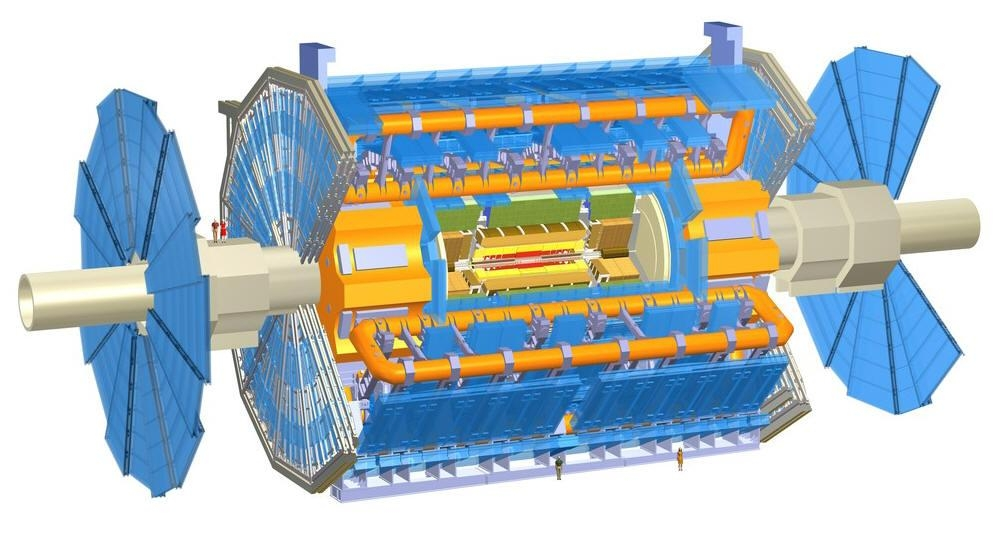
\includegraphics[width=\textwidth]{figures/ATLAS.jpeg}
\caption[The ATLAS detector]{The ATLAS detector apparatus.
\label{fig:thedetector}}
\end{figure}


\begin{description}
	\item[Inner Detector] The inner detector is the first (yellow and red) layer in Figure \ref{fig:thedetector}, and is responsible for measuring the momentum of charged particles. Within the inner detector, we have the Pixel Detector, the Semiconductor Tracker, and the Transition Radiation Tracker.
	
	\item[Calorimeter] The Calorimeter is the green area in Figure \ref{fig:thedetector}, and resolves the energies carried by the particles.
	
	\item[Muon Spectrometer] The Muon Spectrometer is composed of all blue areas in Figure \ref{fig:thedetector}, and is responsible for identifying and measuring the momenta of muons.
	
	\item[Magnet System] The Magnet System is comprised of all orange regions in Figure \ref{fig:thedetector}. It is responsible for bending charged particles in order to measure momentum with higher resolution. 
\end{description}

\section{Software and Data Acquisition Overview}

\newthought{While turned on}, the ATLAS detector reads in 1 Billion particle collisions per second. Most of these events are of no interest, which necessitates systems that are able to syphon through the sea of data. Using a two-level \emph{trigger system}\footnote{A system which makes nearly instantaneous decision about which events to keep and throw away.}, the ATLAS collaboration is able to obtain data on events that have potential for valuable physics contributions. 

\subsection{Trigger}

The trigger is split into the LVL1 and LVL2 triggers. The LVL1 trigger uses basic hardware-level logic to decide on regions of interest within the detector, and keep only data that reaches said regions. It requires about 2 micro-seconds to reach its keep-or-throw decision, including the delays due to cables between the detector and the underground room where the trigger logic is housed. The LVL2 trigger uses information from all levels of the detector, using a finer granularity when deciding what to keep and what to ignore. At this level, a decision about an event is made within 10ms.

\subsection{Reconstruction}

Using fairly simple algorithms and physical formulae, particle momenta, direction, and dynamics can be reconstructed out of the interactions within the detector. In the case of $b$ and $c$ tagging, we are able to obtain meaningful nature and hand-crafted features that carry information about tracks, vertexing, and energy information, among other things. A full discussion of jet reconstruction is beyond the scope of this thesis -- what is important is that these quantities can help us build a classifier that recognizes latent patterns that drive the dynamics we observe in the detector apparatus.

\subsection{ROOT}

All physics objects used within an analysis are stored in formats defined in the ROOT \citep{ROOT} C++ framework. The data we work with in this thesis is stored in a so-called D3PD, which are stored in structures called a \texttt{TTree}. Intuitively, a D3PD is a standard table, where each row can have entries which are arbitrarily sized C++ Standard Library objects. The data we use is stored in such structures, and as will be elaborated upon later in this thesis, we provide a C++ wrapper around the D3PD and \texttt{TTree} interface.


